\section{Signal- und Datenverarbeitung von Mess\-einrichtungen}

Datenerfassung oder auch Datenakquisition (\textit{engl. data acquisition}) wird häufig DAQ abgekürzt. In den folgenden Abschnitten wird die DAQ mittels
\begin{align*}
\mathrm{integrierter\,Messdatenerfassung\,}  &\textrm{via}\, \textbf{RS-232\,} \mathrm{Schnittstelle}, \\
\mathrm{analog\,Signalumwandlung\,mittels\,} \textbf{NI-USB\,6001\,} \mathrm{Messkarte\,} &\textrm{via}\, \textbf{USB\,}\mathrm{Schnittstelle}
\end{align*} 

unter der Verwendung von LabVIEW (2018, 2020) erläutert. Es werden Module programmiert, mit denen man kontinuierliche und diskrete Signalströme und Daten verarbeiten kann. Somit ist es möglich, für alle Unit Operations Masken zu erstellen, in der Daten eingegeben werden können. Diese diskreten Daten  können in einer separaten Datei oder als Header einer z.B. \texttt{Tabulator} getrennten \glqq kontiMessungs.txt\grqq{} Datei gespeichert werden. Man ist nicht daran gebunden als Spaltentrennzeichen (\textit{engl. delimiter}) \texttt{Tabulator} zu verwenden, auch die Verwendung eines \texttt{Komma} (.csv Datei), \texttt{Semikolon} oder auch ein frei wählbares Trennzeichen ist möglich. Aufgrund der internationalen Konventionsunterschiede in Bezug auf das Dezimaltrennzeichen (ASCII \texttt{'.'}, in Deutschland \texttt{','} etc.)  ist von der Verwendung eines \texttt{Komma} jedoch abzuraten.

\paragraph{RS-232 zu USB Adapter} Wenn ein PC keine RS-232 Schnittstelle besitzt, kann ein RS-232 zu USB Adapter verwendet werden. Ein Mikroprozessor im Kabel emuliert eine RS-232 Schnittstelle. \\

\subsection{Serielle Schnittstellenkonfiguration und Signalverarbeitung von Messeinrichtungen}

In diesem Abschnitt werden virtuelle Instrumente (VI) zur Verarbeitung kontinuierlicher und diskreter Daten im ASCII Format (ASCII \textit{encoded}) programmiert, die über eine RS-232 Schnittstelle empfangen werden und die Daten verarbeitet. Auf der Abbildung \ref{fig:sensor_digitale_schnittstelle} ist zu erkennen, wie die hardwareseitige Datenverarbeitung im Falle eines Messgeräts mit integrierter digitaler Schnittstelle aussieht. Das Messobjekt, dass könnte z.B. die Massebestimmung eines Syntheseprodukts sein, wird Messtechnisch mittels Sensor erfasst und transmittiert das im Messgerät bereits umgewandelte Signal an einen Microcontroller, PC oder ähnliches.

\begin{figure}[h!] %[htbp!] 
\centering
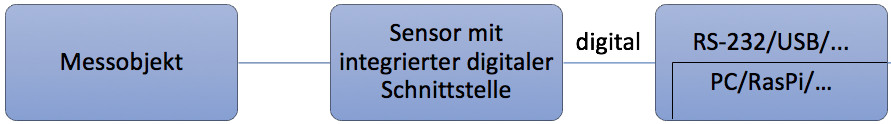
\includegraphics[width=0.75\textwidth]{Bilder/sensor_digitale_schnittstelle.jpg}
\vspace{0em}
 \caption[Messeinrichtungen mit integrierter digitaler Schnittstelle]{Messeinrichtungen mit integrierter digitaler Schnittstelle}\label{fig:sensor_digitale_schnittstelle}
\end{figure}

 Es werden die Schritte erklärt, wie man mit LabVIEW einen kontinuierlichen Datenstrom verarbeitet, der über eine RS-232 Schnittstelle empfangen wird. Es wird ein Windows 10 PC sowie ein Mac Book Pro und LabVIEW 2018 sowie LabVIEW 2020 verwendet, um die VI's zu programmieren und die Signale eines Messinstruments zu verarbeiten. Als Demonstrationsmesssystem wird eine Digitalwaage des Modells 440-47N des Herstellers KERN ausgelesen und die Daten interpretiert, die in eine Tabulator getrennten Text-Datei (*.txt) geschrieben werden. Die Waage hat einen integrierten analog/digital Wandler und besitzt eine RS-232 Schnittstelle. Das Programm wird aus mehreren Sub VI's (siehe Tabelle\,\ref{tab:subvis}) und dem Haupt VI bestehen. \\

\begin{table}[h] % Serielle Konfigurationsparameter der Digitalwaage KERN 440-47N
\caption{Sub VI's}
\begin{center}
\begin{tabular}{r|l}
\onehalfspacing
%\hline
Serial Sub VI \hspace{6pt} & \hspace{6pt} Abbildung: \ref{step5} \\
VTP Elapsed Time  \hspace{6pt} & \hspace{6pt} Abbildung: \ref{fig:vtp_elapsed_time}   \\
Header Module \hspace{6pt} & \hspace{6pt} Abbildung: \ref{fig:modularer_header}  \\
%\hspace{6pt} & \hspace{6pt}  \\

%\hline
\end{tabular}
\end{center}
\label{tab:subvis}
\end{table}


\noindent In einem VI wird der Datenstrom, der von der Waage übermittelt wird, Akquiriert. Das Sub VI wird folgend \textit{Serial Sub VI} oder in der Kurzform \textbf{SSVI} genannt. Das \textbf{Haupt VI} wird die Daten, die es vom Sub VI erhält verarbeiten/interpretieren und in eine *.txt Datei loggen. Des Weiteren soll das Haupt VI einen live plotter besitzen. Für einen modularen Header werden Sub VI's geschrieben, welcher Daten wie Gruppennummer, lokaler (des jeweiligen PC's) Datum- und Zeitstempel (modifizierbar), die VT Praktikums Nr. o.ä. enthält.\\

\noindent Um die korrekte Konfiguration Ihres Geräts vorzunehmen zu können, ist in dem Handbuch des Geräts nach folgenden Parametern zu schauen:

\begin{itemize} % RS-232 Parameter
\singlespacing
\item Zeichen Codierung, z.B. 8-\texttt{Bit} 'ASCII'
\item Baudrate
\item \texttt{Paritätsbit}
\item \texttt{Stopbit}
\item Flusssteuerung (\textit{Flow Control})
\end{itemize}

\noindent Die Digitalwaage sendet ihre digitalen Signale über eine RS-232 Schnittstelle, die 8-\texttt{Bit} ASCII-encodiert sind. Um einen \textbf{kontinuierlichen Datenstrom} zu erhalten und somit \textbf{kontinuierlich} zu Wiegen, wird in der Einstellung der Waage \glqq automatisches Senden\grqq{} eingestellt (das Gewicht soll gesendet werden, auch wenn der Wert nicht stabil ist). Die seriellen Konfigurationsparameter der Waage und des PC's bzw. des verarbeitenden Programms wie z.B. LabVIEW müssen identisch sein, um decodierbare Daten empfangen zu können. Diese Einstellungen sind über das Menü der Waage vorzunehmen. In der Tabelle \ref{tab:kern440} werden die verwendeten seriellen Konfigurationsparameter der Waage 440-47N des Herstellers Kern aufgelistet (Kurzschreibweise in  (\textit{engl. shorthand notation})).

\begin{table}[h] % Serielle Konfigurationsparameter der Digitalwaage Kern 440-47N
\caption{RS-232 Konfigurationsparameter der Digitalwaage Kern 440-47 N in shorthand \\ notation 8-N-1}
\begin{center}
\begin{tabular}{r|l}
\onehalfspacing
%\hline
Baudrate in\,$\mathrm{s}^{-1}$ \hspace{6pt} & \hspace{6pt} 1200 \\
Bytelänge in \texttt{Bit} \hspace{6pt} & \hspace{6pt} \textbf{8}  \\
\texttt{Paritätsbit} \hspace{6pt} & \hspace{6pt} None (\textbf{N)} \\
\texttt{Stopbit} \hspace{6pt} & \hspace{6pt} \textbf{1} \\
Encoded \hspace{6pt} & \hspace{6pt} ASCII \\
FlowControl \hspace{6pt} & \hspace{6pt} Software-Handshake \\
%\hline
\end{tabular}
\end{center}
\label{tab:kern440}
\end{table}

\subsection{Serielle Schnittstelle im Betriebssystem finden und Debuggen} 

Die für den Benutzer sichtbare Benennung des RS-232 Ports unterscheidet sich zwischen den Betriebssystemen. Im Verlauf des Projekts wurde mit einem Unix (Mac Book Pro) und Windows 10 Betriebssystem gearbeitet. 

\paragraph{Microsoft Windows} Bei der Verwendung eines Windows PC's wird der Port der seriellen Schnittstelle Com Port genannt und wird im Gerätemanager und in Programmen wie z.B. LabVIEW COM\texttt{1-N} aufgelistet. 

\paragraph{Mac Unix} Bei der Verwendung eines MACOS/Unix ist die serielle Schnittstelle im Terminal des Mac unter ~dev/tty.* und ~dev/cu.* zu finden und wird in LabVIEW \mbox{ASLR \texttt{1-N}::INSTR} genannt. \\

\noindent Um die richtigen Parameter zu identifizieren oder ob generell Signale und wenn in welcher Form empfangen werden kann mit einigen Tools erreicht werden.

\paragraph{Tool zur Identifikation und Debuggen serieller Schnittstellen} Um herauszufinden ob die Konfigurationsparameter Stimmen, ein Gerät Daten Sendet, wie das Datenformat aussieht und ob die Daten korrekt übermittelt werden, kann man unter Windows ein kostenloses Tool namens hTerm verwenden. Ein etwas weniger komfortables, jedoch vergleichbares open source Tool unter Mac oder Linux ist CoolTerm.\\

\subsection{Kontinuierliche Daten via RS-232 und LabVIEW verarbeiten}

Die grafische Programmiersprache G mit der Entwicklungsumgebung LabVIEW ist in der Lage Daten via RS-232 Schnittstelle zu akquirieren und zu interpretieren. Um eine serielle Schnittstelle in LabVIEW auslesen zu können, wird der \textbf{NI-VISA} Treiber benötigt. 
\vspace{1mm}
\begin{quote}
\footnotesize 
\noindent \textbf{Anmerkung:} NI hat für UNIX/MACOS kein kein Paket Manager vorgesehen. Es werden unter Mac einige Funktionen nicht unterstützt, wie unter anderem der LabVIEW Paketmanager und einige Pakete wie bspw. DAQmx für den Mac zu erhalten und zu implementieren hat \glqq Potentiall\grqq{}. DAQmx konnte nicht auf einem UNIX Betriebssystem eingerichtet werden, somit ist LabVIEW nicht zu 100\% Betriebssystem unabhängig. 
\end{quote}
\vspace{2mm}

\subsubsection{Anpassung der LabVIEW-Einstellungen}
\label{sec:LabVIEW_Einstellungen}

Damit Texteingaben in Eingabefenster (\textit{Control} Fenster) mit der Betätigung von Enter bestätigt/quittiert wird, ist in den LabVIEW Einstellungen folgender Hacken zu setzen:

\begin{center}  % Tools > Options... > Category > Enviroment > End text entry ...
Tools > Options... > Category > Enviroment > End text entry with Enter key [aktivieren]
\end{center} 

\noindent Wenn ein serieller Port geöffnet wird \textbf{ist es wichtig, dass bei dem Beenden des Programms der serielle Port geschlossen wird!} Wenn der Abbruch Button (\textit{engl. abort button}) von LabVIEW genutzt wird, wird der Port nicht geschlossen, daher soll das VI nur über den \textit{Stop Button} des Frontpanels geschlossen werden. Um den \textit{Abort Button} für das gerade verwendete VI (Programm) zu entfernen, gehen Sie bitte wie folgt vor:

\begin{center} % File > VI properties... > Window Apperance > Customize ...
File > VI properties... > Window Apperance > Customize ... >  Show Abort button [deaktivieren]
\end{center} 

\input{Benötigte_LabVIEW_Objekte}
 
\subsubsection{Serielle Sub VI programmierung}

Zu Beginn wird ein VI oder wie auch nachfolgend \textit{Objekt} genannt programmiert (in LabVIEW auf englisch \textit{Function}). Dieses VI wird im folge Abschnitt in das Haupt VI als Sub VI mit dem Namen \textit{Serial Sub VI} integriert. Zu Beginn öffnet man ein neues leeres VI. Das \textit{Serial Sub VI}, im folgenden \textit{SSVI} wird für die Konfiguration einer seriellen Schnittstelle verwendet. Die von LabVIEW verwendeten \textit{Objekte} können Sie den Tabellen \ref{tab:labviewserialobject} und \ref{tab:labviewserialobject2} entnehmen. In den Tabellen \ref{tab:labviewserialobject} und \ref{tab:labviewserialobject2}, die sich ebenfalls im Anhang befinden, sind alle Objekten aufgelistet, die benötigt werden, um die \textit{VI's} zu programmieren. In den Tabellen \ref{tab:labviewserialobject} und \ref{tab:labviewserialobject2} wird das Blockdiagramm mit \textbf{BD}, das Front Panel mit \textbf{FP} und die rechte Maustaste mit \textbf{rM} abgekürzt. In den folgenden Programmierabbildungen sind die Funktion wie in den Tabellen \ref{tab:labviewserialobject} und \ref{tab:labviewserialobject2} nummeriert.\\

\paragraph{Erster Schritt: Serielle Objekte} Nach dem Erstellen eines neuen VI's, fügt man alle Objekte ein, die man für den Datentransfer mit serieller Schnittstelle benötigt (4 - 9 in Tabelle \ref{tab:labviewserialobject}) (siehe Abbildung \ref{step1}). 

\bildp{h!}{1}
{LabVIEW_serialport/step_1_all_serial_functions_2.png}
{0em}
{Einfügen aller seriellen Funktionen}
{Einfügen aller seriellen Funktionen}
{step1}


\paragraph{Zweiter Schritt: Port Initialisierungs- und Abbruchskonfiguration} An dem Objekt \textit{Configure Port} sind Konstanten mit den Konfigurationswerten hinzufügen. An den Objekteingängen auf der linken Seite des Objekts, erstellt man Konstanten (rechte Maustaste/\textit{Create Constant} (11), siehe Abbildung \ref{step2}), die die seriellen Konfigurationsparameter enthalten (siehe Tabelle \ref{tab:kern440}). Um den Anwender dieses VI's den gesamten kombinationsraum der Parameter zu Verfügung zu stellen, ist es auch möglich anstelle der Konstanten, \textit{Controls} zu verwenden (siehe Abbildung \ref{haupt_ini_oben}). Anschließend zieht man eine \textit{Case-Structur} (2a) um das \textit{Configure Port} (zzgl. Konstanten) und das \textit{Flush Buffer} (9) Objekt und eine weitere \textit{Case-Structur} (2b) um das \textit{Close Port} Objekt. Wird die \textit{Case-Structure} (29) mittels eines Wahrheitswerts (\textit{boolean variable}, \texttt{true}/\texttt{false}) getriggert, wird somit der Port Konfiguriert und der I/O Buffer geflushed. Die \textit{Case Structure} (2b), auf der rechten Seite wird mittels eines \textit{Stop Buttons} auf \texttt{true} gestellt, um den Port mittels des \textit{Close} (8) Objekts zu schließen.\\

\noindent Den Stop \textit{Button} (14), die \textit{VISA ressource name} (13) zur Auswahl des Ports und den String \textit{Indicator} (12) (siehe Tabelle \ref{tab:labviewserialobject}, 12 - 14) fügt man z.B. über das Front Panel hinzu und positioniert die dazugehörigen Objekte, die automatisch im Blockdiagramm erscheinen, an der richtigen Positionen. Der \textit{Stop Button} wird mit dem \textit{Case Selektor} der zweiten \textit{Case-Structure} (2b) verbunden. Wird das Programm durch diesen \textit{Stop Button} beendet, wird somit der Port geschlossen. \textbf{Aufgrund dessen ist es wichtig, den VI Abbruch Button zu Deaktivieren: \emph{File > VI properties... > Window Apperance > Customize ... > [Markierung entfernen] Show Abort button}}. Ein \textit{Indicator} zum Anzeigen und zum weiter reichen des, durch das \textit{Read} Objekt (6) ausgelesenen Strings, wird an das \textit{Read} Objekt (6) angeschlossen. Die erste \textit{Case Structure} (2a) wird durch ein \textit{First Call?} (3) Objekt getriggert.\\

\begin{figure}[hp!]
\subfloat
	[Einfügen von Stop Button, Indicators und VISA resource]
	[Einfügen von Stop Button, Indicators und VISA resource \label{step2}]{
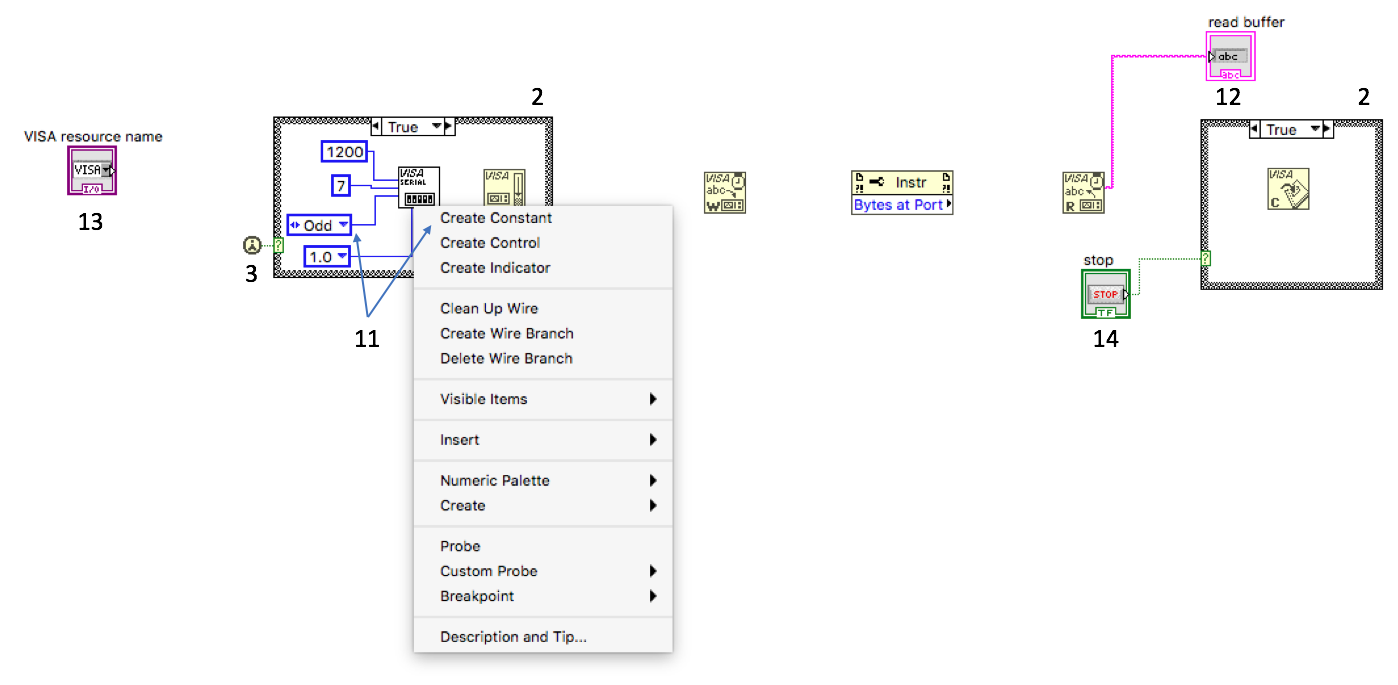
\includegraphics[width=1\textwidth]
	{Bilder/LabVIEW_serialport/step_2_cases_buttons-indicators-controls_2.png}
}
\phantomcaption
\vspace{5pt}
\ContinuedFloat
\subfloat
	[Einfügen von For Loop und Schieberegister]
	[Einfügen von For Loop und Schieberegister\label{step3}]{
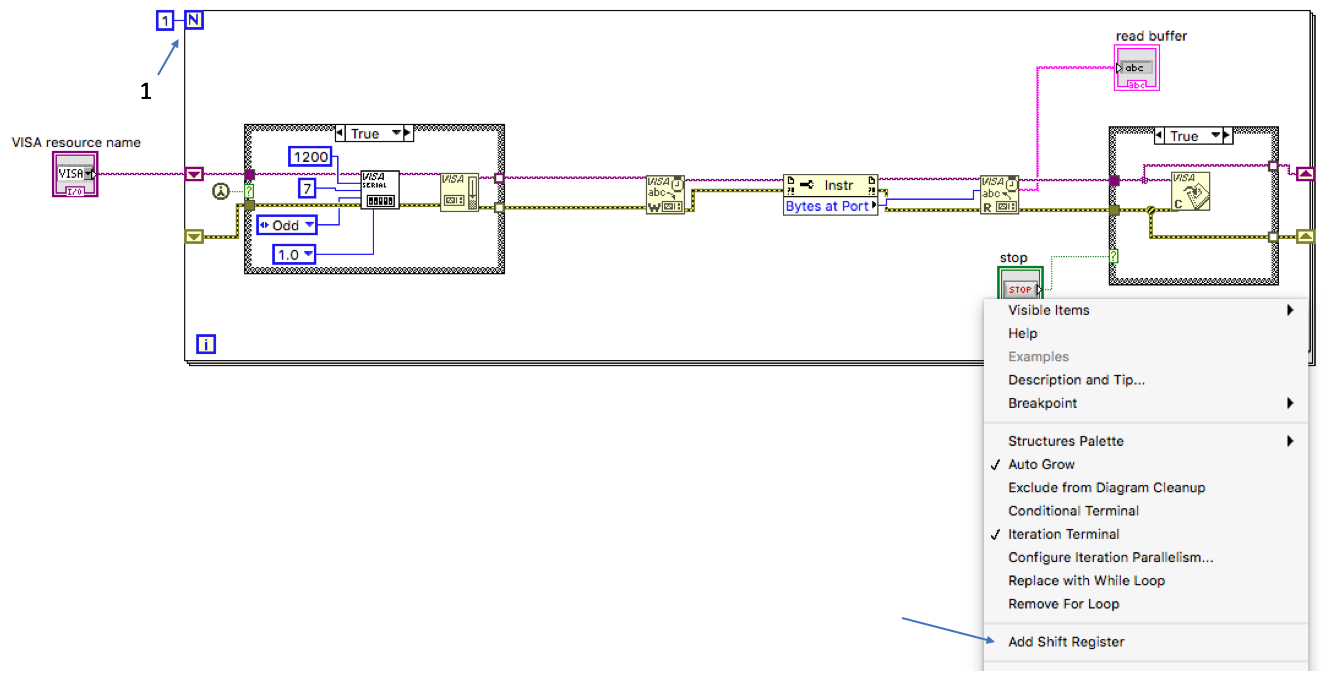
\includegraphics[width=1\textwidth]
	{Bilder/LabVIEW_serialport/step_3_for-loop_add-shift-register_2.png}
} 
\caption[]{Einfügen von Stop Button, Indicators, VISA resource, For Loops und Schieberegister}
\label{fig:step2_step3}
\end{figure}


\paragraph{Dritter Schritt: N = 1 For Loop, XON flow control}

Nun zieht man ein eine \textit{For Loop} um alle Objekte, bis auf die \textit{VISA Resource} und das \textit{Flush Buffer} Objekt. Die \textit{For Loop} wird in diesem Fall mit der Konstante 1 initialisiert (siehe Abbildung \ref{step3}, oben links). Nach dem hinzufügen von zwei Schieberegistern (\textit{engl. Shift Register}), sind alle Objekte wie in Abbildung \ref{step3} zu verdrahten. Durch das Hinzufügen eines \textit{Shift Registers} an einem Ende einer \textit{For Loop} oder \textit{While Loop}, werden automatisch die \textit{Shift Register} auf der anderen Seite des Loops generiert. Alle Funktionen müssen nun, wie in Abbildung \ref{step3}, verbunden werden (die blaue Leitung zwischen \textit{Bytes at Port} und \textit{Read Port} ist ebenfalls zu verbinden). Da die \glqq Verkabelung\grqq{} im \texttt{true} Case beider \textit{Case Structures} verkabelt sind, muss selbiges noch im \texttt{false} Case beider \textit{Case Structures} (2ab) geschehen (siehe Abbildung \ref{step3b}). Das \textit{Write} Objekt (7) ist mit der String Konstante (10) mit dem Wert \texttt{11} zu verknüpfen. Die \textit{String Konstante} 11 beinhaltet das ASCII flow control (siehe Abschnitt RS-232) Signal XON und signalisiert der Waage, dass der PC bereit ist Daten zu empfangen, da die KERN Waage als flow control den Software-Handshake verwendet. Technisch wird an die Waage der Hexadezimale \textit{character} 11 geschickt, also \texttt{0x11}. \texttt{0x11} ist das ASCII Hexadezimalzeichen für XON (siehe Tabelle \ref{ascii_table} im Anhang).  Dieses Objekt in dieser Form ist nun alleinstehend fähig den seriellen Port zu konfigurieren, der Waage das \textit{flow control} Signal XON zu senden, die Bytes Auszulesen und Darzustellen oder dem Haupt VI zu übergeben sowie den seriellen Port zu schließen, wenn das Programm über den stop Button beendet wird.

\begin{figure}[h!p]
	\hfill     
     \subfloat[\glqq Verdrahtung\grqq{} der \texttt{false} Cases]
     [\glqq Verdrahtung\grqq{} der \texttt{false} Cases\label{step3b}]{%
       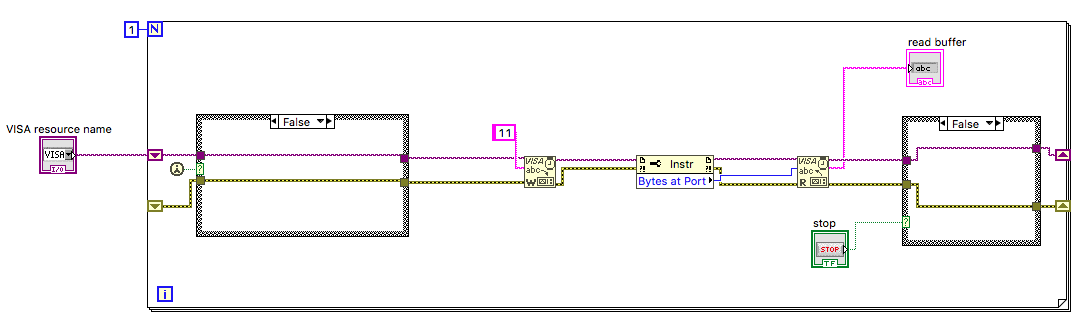
\includegraphics[width=0.99\textwidth]
       {Bilder/LabVIEW_serialport/step_3b_false_cases.png}
     }
     \phantomcaption
     \vspace{3pt}
\ContinuedFloat  
     \subfloat[Einfügen von For Loop und Schieberegister]
     [Optimiertes SSVI\label{step5}]{%
       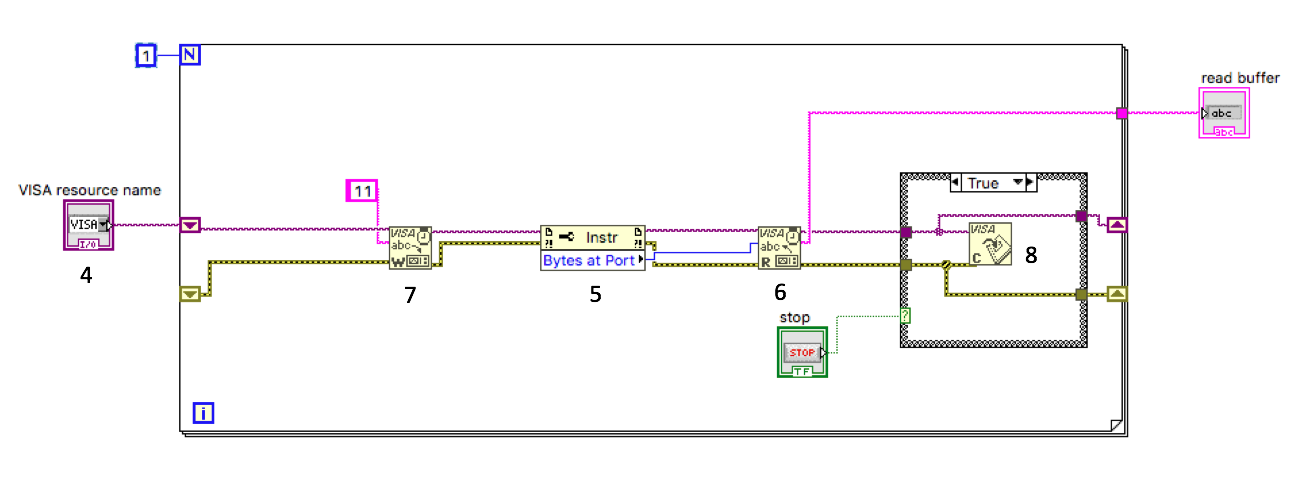
\includegraphics[width=1\textwidth]
       {Bilder/LabVIEW_serialport/step5_optimierung.png}
     }
     \caption[]{\glqq Verdrahtung\grqq{} der \texttt{false} Cases und Optimiertes SSVI
  }
  \label{fig:step3b_step5}
\end{figure} % Einfügen von Stop Button, Indicators, VISA resource, For Loops und Schieberegister



\paragraph{Vierter Schritt: Optimierung} Das Programm in Abbildung \ref{step3} und \ref{step3b} konfiguriert bei jeder Iteration den Port und öffnet ihn. Das öffnen eines seriellen Ports, der bereits geöffnet ist, kann zu Störungen führen, daher sollte die Konfiguration des Ports über das Haupt-VI erfolgen. Der I/O-Buffer soll auch nur bei der ersten Iteration des Hauptprogramms gelöscht werden, der wird ebenfalls ins Haupt VI verlagert. In Abbildung \ref{step5} ist das Objekt nach der Optimierung abgebildet. Um den ausglesenen String nach Abschluss der Iteration an das Haupt VI übergeben zu können, wird der read Buffer rechts aus die For Loop geleitet. Das Objekt \textit{Configure Port} hat für den Inputbuffer per default 4096 \texttt{Bytes} (Anmerkung: Sollte Ein I/O Buffer overflow o.ä. auftreten, dann könnte die Pause zwischen Iterationen zu lang sein). Mit Abschluss dieser Schritte ist das VI Objekt einsatzbereit und kann in mehrere Programmen, implementiert werden. Dafür müssen in der oberen rechten Ecke des Frontpanels die Ein- und Ausgänge des VI festgelegt werden (siehe Abbildung \ref{step4}, Nr. 16). Dazu klickt man auf ein Feld des Icons in der oberen rechten Ecke und auf eine Funktion, die sich im Frontpanel befindet. In diesem Beispiel wurde die obere rechte Ecke des mini Icons angewählt und mit einem Klick auf \textit{read buffer}, dem ausgelesenen String zugeordnet. Die obere linke Ecke des mini Icons wird mit VISA resource name und die Ecke unten links mit dem \textit{Stop Button} belegt.

\bild{.4}
{LabVIEW_serialport/step_4_VI_generieren_3.png}
{0em}
{Definition der VI Objekt Ein- und Ausgänge}
{Definition der VI Objekt Ein- und Ausgänge}
{step4}


\subsubsection{Kontinuierliche Messdatenerfassung RS-232 Haupt VI}

Die Daten, die man via RS-232 empfängt, müssen interpretiert und in einer *.txt Datei gelogged werden. Die empfangenen Daten hängen von der verwendeten Messtechnik ab. Das Untersuchungsobjekt im Rahmen dieses Abschnitts ist eine Digitalwaage (KERN 440-47N). Das Datenformat dieser Waage ist wie folgt:

\begin{enumerate}
\singlespacing
\item Es können beliebig viele Leerzeichen zu Beginn des Strings vorhanden sein (\texttt{'\textbackslash s'})
\item Es kann die Vorzeichen \texttt{+} oder \texttt{-} enthalten
\item Es können beliebig viele \texttt{'\textbackslash s'} folgen
\item Es können beliebig viele Ziffern folgen
\item Es wird ein dezimal Trennungszeichen folgen (ASCII encodiert wäre es der Punkt \texttt{'.'})
\item Es können wieder unbekannt viele Ziffern folgen
\item Es können beliebig viele \texttt{'\textbackslash s'} folgen
\item Es kann die Maßeinheit \texttt{'g'} folgen, wenn der Messwert stabil ist
\item Es können beliebig viele \texttt{'\textbackslash s'} folgen
\item Das Zeilenende kann je nach System variieren. Es kann \texttt{'\textbackslash r'}, \texttt{'\textbackslash n'}, \texttt{'\textbackslash r''\textbackslash n'} oder \texttt{'\textbackslash r\textbackslash n'} sein
\end{enumerate}


\paragraph{Erster Schritt: Port Konfiguration und String verketten/Anzeigen lassen} Nach dem Erstellen eines neuen, leeren VI's, wird das VI des vorherigen Abschnitts per drag and drop in das leere VI gezogen. Dazu zieht man das Symbol 16 des \textit{SSVI} (siehe Abbildung \ref{step4}) in das neue VI. Als nächstes setzt man eine While Loop um dieses VI Objekt und verknüpft einen Stop Button (14) mit dem Stop Eingang des SSVI sowie dem Abbruchkriterium der While Loop (20). Außerhalb des Loops wird die Portkonfiguration (siehe Tabelle \ref{tab:kern440}) und das Objekt, welches den I/O Buffer (9) löscht, platziert. Um die Daten der Waage in Form eines Strings aus dem SSVI auszulesen, wird die Funktion zum Verketten von Strings \textit{engl. Concatenate Strings} (17) in den Loop platziert. Man benötigt Schieberegister (\textit{engl. Shift Register}), erweitert das \textit{Concatenate Strings} (17) Objekt auf zwei Eingänge und verbindet die \textit{Shift Register} mit der \textit{Concatenate Strings} (17) Funktion (links oberer Eingang des \textit{Concatenate Strings} (17) Objekts). Damit das \textit{Shift Register} bei der ersten Iteration (Index = 0, da LabVIEW, wie viele andere Programmiersprachen, 0 indiziert arbeitet) leer ist, wird das linke \textit{Shift Register} mit einer leeren String konstante gelöscht. In Abbildung \ref{step6} sind die beschriebenen Funktionen abgebildet. Um zu sehen ob und was empfangen und verkettet wird, fügen wir einen \textit{String Indicator} (21) ein. Da der Nutzer des Programms \textit{VISA Ressource} und \textit{String Indicator} sehen wird, ist es empfehlenswert es im FP in etwas eindeutiges umzubenennen. Um eindeutig erkennen zu können, welche Zeichen empfangen werden, kann man im Front Panel per rechts-klick in das entsprechende Fenster, die \textit{String Indicator} Anzeige in \texttt{'\textbackslash'} umstellen (siehe Abbildung \ref{step6b}).

\bildp{h!}{1}
{LabVIEW_serialport/step6.png}
{0em}
{BD Haupt VI: SSVI Integration/Port Konfiguration/String\-operationen}
{BD Haupt VI: SSVI Integration, Port Konfiguration, String auslesen und \mbox{verketten}}
{step6}



\bild{0.4}
{LabVIEW_serialport/step6b.png}
{0em}
{FP Haupt VI: SSVI Integration/Port Konfiguration/String\-operationen}
{FP Haupt VI: SSVI Integration, Port Konfiguration, String auslesen und \mbox{verketten}}
{step6b}

\paragraph{Zweiter Schritt: \glqq String Slicing\grqq{}} Das VI verkettet den String bis zum Beenden des Programms. Um eine einzige abgeschlossene Zeichenkette (von String Beginn bis \texttt{'\textbackslash n'}) zu erhalten, müssen wir den String kürzen (\textit{engl. slicing}). Dazu wird eine \textit{Case Structure} (2c) programmiert, die den String verkettet, bis die \textit{Search/Split String} (23) Funktion das von uns gesuchte Zeichen, das ASCII Steuerzeichen \texttt{'\textbackslash n'} liest. Es können zwei Zustände vorliegen, \texttt{true} und \texttt{false}. 

\begin{quote}
Anmerkung: Bei der Funktion \textit{Configure Port} (4) ist per default \textit{Termination Character} auf \texttt{true} gesetzt, was dazu führt, dass \textit{Read} (6) des SSVI beim decodieren der bytes, die sich im Input Buffer des Serial Ports befinden, beim decodieren des Steuerzeichens\texttt{ '\textbackslash n'}, die Zeichenkette terminiert und alle weiteren Bytes, die sich im Input Buffer befinden, in der nächsten Iteration bis maximal zu einem \texttt{'\textbackslash n'} gelesen und decodiert werden.
\end{quote}


\paragraph*{false} Die \textit{Search/Split String} Funktion soll nach einem \texttt{'\textbackslash n'} Suchen. Der \textit{offset of match} Ausgang der Funktion gibt den Index des Matches im String an. Wenn die \textit{Search/Split String} Funktion das zu suchende Zeichen (in dieser Situation\texttt{ '\textbackslash n'}) nicht findet, gibt \textit{offset of match} -1 wieder. Diese Information wird genutzt, um den \textit{Case Selektor} auf \texttt{false} zu setzen. 

Wenn der String kein \texttt{'\textbackslash n'} enthält, gibt die Funktion als \textit{offset of match} den Index -1 zurück, demnach ist das boolsche Signal \texttt{true} aus der \textit{Equal?} (26) Funktion. Dieses Signal wird mit dem boolschen Operator \textit{Not} (27) negiert. Der \textit{Case Selector} (24) ist somit auf \texttt{false} gesetzt.\\
Ist der \textit{Case Selector} (24) auf \texttt{false}, wird der Draht, der den verketteten String (\textit{Shift Register} und \textit{SSVI}) enthält, in die \textit{Case Structure} (2c) geleitet und mit dem rechten \textit{Shift Register} verbunden.\newline

\noindent An dieser Stelle (siehe Abbildung \ref{slicing_bedingung}) wird nun eine \textbf{Sicherheit} eingebaut. Der String soll erst interpretiert werden, wenn die Länge des Strings größer einer Vorgabe ist. Die Länge einer Zeile kann dem Handbuch des jeweiligen Geräts entnommen werden oder sie wird durch das manuelle \textit{Debugging} z.B. hTerm oder trial and error eruiert. 


\begin{figure}[h!] 
\centering
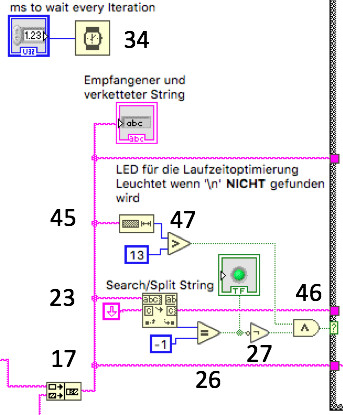
\includegraphics[width=0.35\textwidth]{Bilder/LabVIEW_serialport/slicing_bedingung.jpg}
\vspace{2pt}
\caption[Slicing Bedingung]{Slicing Bedingung}\label{slicing_bedingung}
\end{figure}

\paragraph*{true} Wenn der String \texttt{'\textbackslash n'} enthält, gibt \textit{offset of match} dem \textit{Search/Split String} (23) Objekt den Index an, wo das Zeichen (in diesem Fall \texttt{'\textbackslash n'}) im String gefunden wurde. Der ist ungleich -1, der boolsche Zustand ist somit \texttt{false} und wird mit der \textit{Not} (27) Funktion wieder in ein \texttt{true} umgewandelt. Der \textit{Case Structure Selector} (24) ist damit auf \texttt{true} gesetzt. Nun soll der Folgeiteration der Teil des Strings ab dem gesuchten Zeichen übergeben werden. Das kann mithilfe des Objekts \textit{String Subset} erreicht werden, indem man den Rest des Strings, des Objekts \textit{Search/Split String} (23), im \texttt{true} Case, dem Objekt \textit{String Subset} (25) übergibt. Das Objekt \textit{String Subset} (25) wird die Konstante 1 der Funktion \textit{offset} zugewiesen. Durch diese Konfiguration der Funktionen wird der Rest des Strings \textbf{nach} dem gesuchten Zeichen (\texttt{'\textbackslash n'}) dem \textit{Shift Register} (19) übergeben. Ist der PC und das Programm schneller als die empfangenen Daten, dann ist der übergebene String leer.

 \bild{1}
{LabVIEW_serialport/step7_stringslicing.jpg}
{-1em}
{\glqq String Slicing\grqq{}: Dateninterpretation}
{\glqq String Slicing\grqq{}: Dateninterpretation}
{step7}

\paragraph{Dritter Schritt: \glqq Dateninterpretation\grqq{}} Sobald eine vollständige Zeichenkette gelesen wurde, müssen die Daten in ihre Bestandteile zerlegt werden (siehe Abbildung \ref{step7}). In der \textit{Case Structure} (2c) wird im \texttt{true}\, Case mit dem Objekt \textit{Regular Expression Match} (28), aus dem gesamten vorgelegten String alle gewünschten und potentiell vorkommenden Ausdrücke (\textit{engl. expressions}) separat extrahieren. In der folgenden Liste sind die Ausdrücke (\textit{engl. Submatches}) Aufgelistet, die der String enthält, bzw. enthalten könnte.

\begin{itemize} % Submatch Expression
\singlespacing
\item Es kann ein \texttt{'+'} oder \texttt{'-'} enthalten
\item Beliebig viele \texttt{'\textbackslash s'} (Leerzeichen)
\item Beliebig viele Ziffern
\item Dezimaltrennzeichen (unter ASCII \texttt{'.'})
\item Beliebig viele Ziffern
\item Beliebig viele \texttt{'\textbackslash s'}
\item Es kann ein \texttt{'g'} enthalten sein
\item Beliebig viele \texttt{'\textbackslash s'}
\end{itemize}


 In der folgenden Liste werden die verwendeten \textit{Regular Expression} Operatoren erklärt.

\begin{itemize} %Submatch Expression Operatoren
\singlespacing
\item \texttt{(}x\texttt{)} generiert ein Submatch des Ausdrucks x
\item x\texttt{?} der Ausdruck x kann null oder einmal vorkommen
\item x\texttt{*} der Ausdruck x kann null oder viele male vorkommen
\item \texttt{\textbackslash d+} es können beliebig viele Ziffern (\textit{engl. digits}) vorkommen
\item \texttt{[}...\texttt{]} erstellt eine Zeichenklasse, die Angabe von \texttt{[}xyz\texttt{]} bedeutet, es kann x, y oder z vorkommen
	\begin{itemize} 
		\item[\small $\circ$] sollen Elemente der Zeichenklasse mehrfach vorkommen dürfen, dann ist \texttt{[}...\texttt{]} ein \texttt{+} nachzustellen, daraus folgt \texttt{[}xyz\texttt{]+} 
\end{itemize}
\end{itemize}

\noindent Dem Objekt \textit{Regular Expression Match} müssen wir folgenden Ausdruck in einer String Konstanten mitteilen, die drei Submatches generiert.

\begin{center} %Submatch Expressions
\texttt{
\textbackslash s*([\textbackslash +-])?\textbackslash s*(\textbackslash d+\textbackslash .\textbackslash d+)\textbackslash s*(g?)\textbackslash s*
}
\end{center}

\begin{description}  % Submatches
\singlespacing
\item[Submatch 1] ([\textbackslash +-)?
\item[Submatch 2] (\textbackslash d+\textbackslash .\textbackslash d+)
\item[Submatch 3] (g?)
\end{description}

\noindent Nun ist eine Stringzeile zu Konstruieren (siehe Abbildung \ref{step7}). Das Ziel ist eine *.txt Datei, bei der die Spalten durch das \texttt{Tabulator} Steuerzeichen (\texttt{'\textbackslash t'}) (32) getrennt werden. \textbf{Beim Import einer, mit diesem Programm generierten, Ta\-bu\-lator-getrennt.txt-Datei in, z.B. ein Tabellenkalkulationsprogramm, wie Excel, ist als Spaltentrennzeichen Tabulator anzugeben.} Für die Konstruktion (Verkettung von Strings) einer Zeile verwendet man das \textit{Concatenate} (17) Objekt. Ein String wird in einer textbasierten Programmiersprache wie Python mit Anführungsstrichen (\texttt{''}) deklariert. Das Objekt \textit{Concatenate} verkettet Strings.

\begin{center}
\textit{Concatenate} (17) bewirkt folgendes: \mbox{(\mbox{'ich bin'} + \mbox{'ein String'} = \mbox{'ich bin ein String'})}
\end{center}  

\noindent LabVIEW's \textit{Read} (6) Objekt liest \texttt{Bit}-seriell vom Port, versendet nach dem Lesen \texttt{Byte} seriell. Eine von der Waage gesendete Zeile könnte wie folgt aussehen:

\begin{figure}[h!] %Waagen String vor LabVIEW
\centering
\begin{BVerbatim}
'\s''\+''\s''\s''\s''\s''12''\.''8''\s''g''\s''\r''\n'
\end{BVerbatim}
\end{figure}


\noindent Bei dem \textit{Configure Port} Objekt (4) ist per default\textit{ Termination Character} auf\, \texttt{true} gesetzt, d.h. \textit{Read} (6) liest bis zu einem\, \texttt{'\textbackslash n'}. Der Rest verbleibt für die folgenden Iterationen im Input Buffer. Eine vollständig von \textit{Read} (6) gelesene Zeile ergibt somit folgenden String:


\begin{figure}[h!] %Waagenstring nach LabVIEW
\centering
\begin{varwidth}{\linewidth}
\begin{verbatim}
'\s\+\s\s\s\s12\.8\sg\s\r\n'
\end{verbatim}
\end{varwidth}
\end{figure}


\noindent Nun sollen die drei potentiellen Bestandteile (\texttt{ '+' }, \texttt{ '12.8' }, \texttt{ 'g' }) extrahiert werden. Das Vorzeichen und der Character \texttt{'g'} können, müssen aber nicht vorkommen. Die drei Submatches sind somit: 
\vspace{-2pt}
\begin{center}  \texttt{ '+/-' },\texttt{ '12.8' },\texttt{ 'g' } \end{center}

\noindent Mit den drei Elementen soll eine Datalogger Zeile generiert werden. Die Zeile soll wie folgt aufgebaut sein.

\begin{figure}[h!] %Spaltenformatierung
\begin{center}
\begin{varwidth}{\linewidth}
\begin{verbatim}
  Zeitstempel \t Messwert \t Einheit in g \t Versuchsbeobachtung \n
\end{verbatim}
\end{varwidth}
\end{center}
\end{figure}

\paragraph{Vierter Schritt: Zeilenkonstruktion} Das Programm wird Zeile für Zeile den Inhalt, der in die Tabgetrennte.txt Datei geschrieben werden soll, vorerst als String verketten. Dieser String wird nach dem Stoppen des Programms in die *.txt Datei geschrieben. Für die Konstruktion einer String Zeile wird das \textit{Concatenate} (17) Objekt genutzt (siehe Abbildung \ref{fig:String-/Zeilenkonstruktion}). Eine Dataloggerzeile wird in dieser Konfiguration (17, 22a, 31, 10b, 32, 33 und 29a), wie im vorherigen Abschnitt gefordert, konstruiert. Die Versuchsbeobachtungen werden mittels \textit{Control} (22a) dem jeweiligen Zeitstempel zugeordnet. Nach dem Schreiben in die *.txt Datei muss die \textit{Control} (22a) mit einem leeren String gelöscht werden (siehe Abschnitt \ref{sec:Datalogger} Abbildung \ref{datalogger}). Die verkettete Zeile ist einem \textit{Control} mittels einer lokalen Variable dem \textit{Variablenspeicher 1} (29a) zu übermitteln. Mit der Information, die im \textit{Variablenspeicher 1} hinterlegt wird, ist das kontinuierliche Loggen in eine *.txt, mit \texttt{'\textbackslash t'} als delimiter möglich.

\begin{figure}[h!] % String-/Zeilenkonstruktion
	\centering
	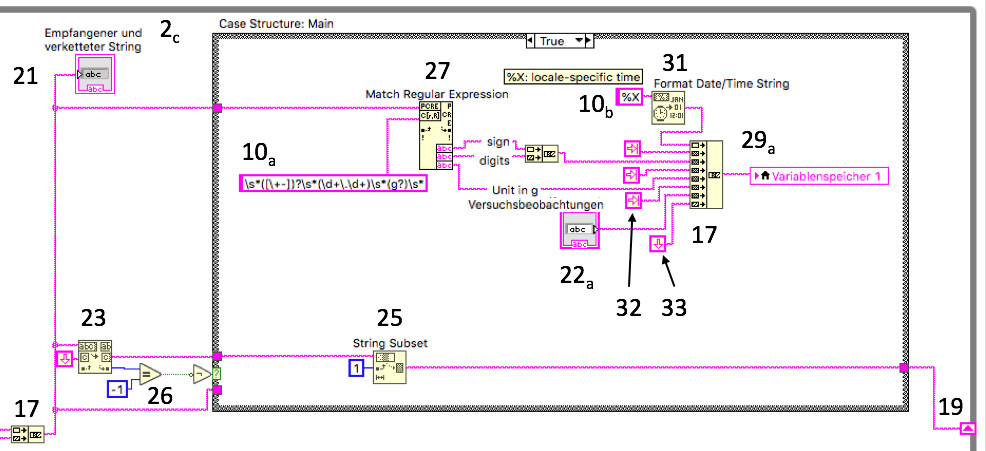
\includegraphics[width=1\textwidth]{Bilder/LabVIEW_serialport/stringkonstruktion.jpg}
	\vspace{2pt}
	\caption[String-/Zeilenkonstruktion]{String-/Zeilenkonstruktion}
	\label{fig:String-/Zeilenkonstruktion}
\end{figure}


\paragraph{Fünfter Schritt: Zeitstempel oder Zeitreihen Programmierung}  Der Zeitstempel (\textit{engl. Time\-stamp}) kann durch die folgenden zwei Methoden implementiert werden. Bei der ersten Methode wird mittels des Objekts \textit{Format Date/Time String} (siehe Abbildung \ref{fig:String-/Zeilenkonstruktion} (31) und (10b)) eine frei formatierbare Zeitreihe möglich (für genauere Infos schauen Sie bitte in \cite{zeitreihenformatierung}). \\

\noindent Um als Zeitstempel die verstrichene Zeit in ms zu bekommen, ist das Objekt wie auf der Abbildung \ref{fig:vtp_elapsed_time} zu Programmieren (VTP Elapsed Time Sub VI) (44). 

%%=================================================================================

\input{Benötigte_LabVIEW_Konfigurationsfunktionen_Teil_2}

%%=================================================================================
 

\begin{figure}[!ht] %Methode 2   simple Elapsed Time in ms Sub VI (37)
     \subfloat[][\texttt{true}\label{fig:true}]
     {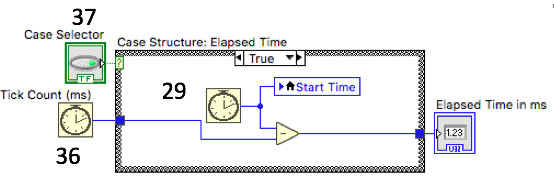
\includegraphics[width=0.5\textwidth]
       {Bilder/LabVIEW_serialport/step7_elapsed_true.jpg}
     }
     \hfill     
     \subfloat[][\texttt{false}\label{fig:false}]
     {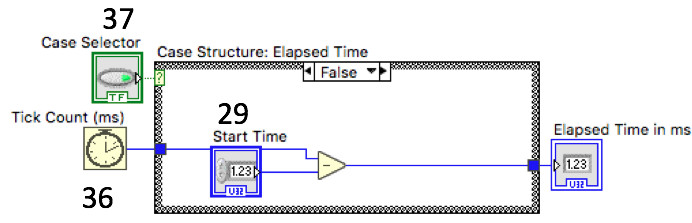
\includegraphics[width=0.5\textwidth]
       {Bilder/LabVIEW_serialport/step7_elapsed_false.jpg}
     }
     \caption[]{Methode 2 \glqq VTP Elapsed Time in ms\grqq{} Sub VI (37)\\     	
  }
  \label{fig:vtp_elapsed_time}
   \end{figure}


\paragraph{Sechster Schritt: Versuchsbeobachtungen} Es ist eine Kommentarfunktion gewünscht. Das Kommentar soll eingegeben werden können und nach der Bestätigung der Eingabe mit\, \texttt{Enter}, soll das Kommentar zum Zeitpunkt der\, \texttt{Enter} betätigung dem jeweiligen Zeitstempel zugeordnet werden. Dafür ist die Einstellung gemäß Abschnitt \ref{sec:LabVIEW_Einstellungen} vorzunehmen. Ein \textit{\textbf{Control}} Objekt (22) kann als Variablenspeicher interpretiert werden. Nach der Übergabe eines Wertes an das \textit{Control} Objekt des Kommentar muss diese nach der Ausgabe wieder gewiped werden. Zum \glqq löschen\grqq{} der letzten Eingabe in \textit{Control} Objekten, ist diese mit einer leeren Stringkonstanten zu überschreiben (siehe Abbildung \ref{datalogger} ) 29a. Der Programmablauf wäre dann wie folgt:


\begin{itemize} % Versuchsbeobachtungsreset
\singlespacing
\item Versuchsbeobachtung wird Eingegeben (22a)
\item \textit{Case Selektor} wird getriggert durch Programmstart oder wenn die Dauer für ein Messwertaufnahmeintervall verstrichen ist
\item sobald der Datalogger Case Selektor getriggert wird, schaltet die \textit{Case Structure} auf \texttt{true}
\item Löschen der \textit{Control Versuchsbeobachtung} durch die Lokale Variable (298) 
\end{itemize}


\paragraph{Siebter Schritt: Dataloggerprogrammierung}
\label{sec:Datalogger}

Die Messwert sollen in eine \texttt{Tabulator} getrennte *.txt geschrieben werden. Als nächstes ist ein Datalogger zu programmieren (siehe Abbildung \ref{datalogger}). Mit den Objekten 38 bis 42 kann ein Datalogger programmiert werden, der jede \textit{While Loop} Iteration die Daten in ein *.txt schreibt, die er in der jeweiligen Iteration übergeben bekommt. Während einer Iteration, kann er beliebig viele Zeilen in die *.txt Datei schreiben. Im \texttt{true} Case wird der String aus \textit{Variablenspeicher 1} in die *.txt Datei geschrieben, die in 40b, vor Programmausführung zu benennen ist (test\_aller\_Funktionen\_Beispiel.txt). Mit dem \textit{Elapsed Time} Objekt (35) kann ein \textit{Control} Objekt Programmiert werden, mit dem das Wertaufnahmeintervall in s eingestellt werden kann. Diese wird der Funktion \textit{Time Target (s)} des \textit{Elapsed Time} (43) Objekts verbunden. Über diese Control kann man das Messwertaufnahmeintervall varieren, auch während des Programmablaufs. Der \textit{Time has Elapsed} boolsche Ausgang ist mit einem \textit{Or} (46) zu verbinden \textit{Case Selector}. Wenn der Iterations Index 0 oder die angegebene Zeit verstrichen ist, wird ein Messwert gelogged, bzw. alle Zeile in die *.txt Datei geschrieben, die dem \textit{Write to Text File} (38) Objekt übergeben wird. Im \texttt{false} Case soll nix passieren, daher werden die Tunnel (insgesamt 2 x 2) beider \textit{Case Structure} Seiten mit einander verbunden. Der \textit{Variablenspeicher 1} wird mit einem leeren String gelöscht (\textit{engl. wiped}, umgangsprachlich gewiped). Damit ist der \textit{Variablenspeicher 1} bis zur nächsten Eingabe geleert.

\bild{1}
{LabVIEW_serialport/step8_datalogger.jpg}
{-1em}
{Datalogger}
{Datalogger}
{datalogger}



\paragraph{Achter Schritt: Modulare Header}

Auf der Abbildung \ref{fig:modularer_header} sind Headermodule (a),(b) und (c) und die Methode, wie man diese mittels \textit{Concatenate} (17) Verkettet. Der Datalogger Header ist somit einfach zu modifizieren.

%\newpage
\begin{figure}[h] % Headerkonfiguration  standardheader Zeile und Zeitreihenheader
     \subfloat[][Erste Header Zeile\label{fig:standard_header}]{%
       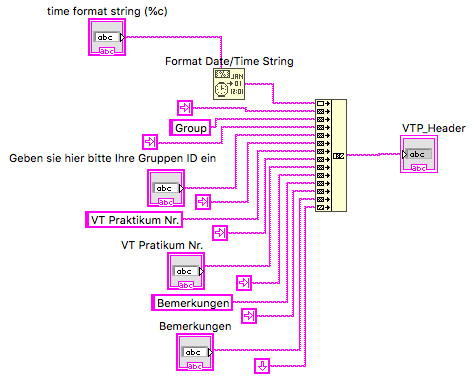
\includegraphics[width=0.5\textwidth]
       {Bilder/LabVIEW_serialport/standard_header.jpg}
     }\hfill     
    \subfloat[][Zeitreihen Überschrift\label{fig:header}]{%
       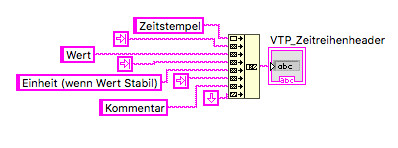
\includegraphics[width=0.5\textwidth]
      {Bilder/LabVIEW_serialport/header.jpg}
     }\phantomcaption
     %\caption[]{}
%  \label{fig:simple_elapsed_time}
   \end{figure}
\begin{figure}[h] % Headerkonfiguration 2 Masse Dokumentenheader
\ContinuedFloat
\subfloat[][Masse Header Zeile\label{fig:vtp_masse}]{%
       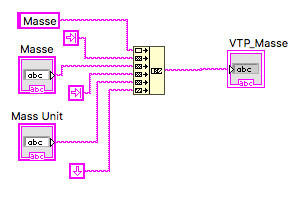
\includegraphics[width=0.5\textwidth]
       {Bilder/LabVIEW_serialport/masse.jpg}
     }\hfill     
    \subfloat[][Verkettung der Headermodule\label{fig:dokumentenheader}]{%
       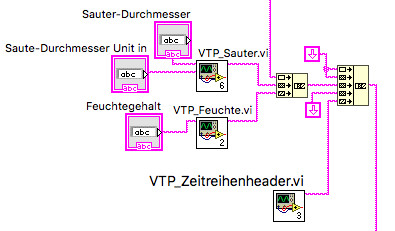
\includegraphics[width=0.5\textwidth]
      {Bilder/LabVIEW_serialport/Dokumentheaderverkettung.jpg}
     }    
\caption[Modulare Header Sub VI's]{Modulare Header Sub VI's}
\label{fig:modularer_header}
   \end{figure}

\paragraph{Neunter Schritt: Auslastungsoptimierung} Um die optimale Programmtaktrate empirisch zu ermitteln, kann man eine \textit{LED} (30) zwischen den Objekten \textit{Equal?} (26) und \textit{Not} (27) platzieren. Nun variiert man die Taktrate der \textit{While Loop} des  \textit{Haupt VI's}, bis die \textit{LED} für die Optimierung blinkt, um Daten \textit{Just in Time} zu erhalten. Das Blinken signalisiert, dass der (Read Buffer) der Datenquelle nicht überfüllt wird. Damit ist gewährleistet, dass für das Ausführen des Programms \textbf{ nur soviel Rechenkapazität verwendet wird wie nötig!} Um die Taktrate rechnerisch zu ermitteln, benötigt man die zu erwartenden \texttt{Bytes}, bzw. Character pro Zeile. Die Baudrate (Bd) gibt an, wie viele \textbf{Zeichen} pro Sekunde versendet werden. In vielen fällen wird für 1\,\textbf{Zeichen},
\,1\,\texttt{Bit} benötigt, daraus folgt, dass die Baudrate in diesen Fällen \texttt{Bit} pro s bedeutet.\\

Mit dem Objekt \textit{wait (ms)} (34) kann man eine Wartedauer (\textit{engl. sleep}) vor jeder Iteration. Mit dem Objekt \textit{wait until next ms multiple} (35) kann man eine Taktzeit für einen Iteration einprogrammieren. Die \textit{sleep} Dauer sollte geringer sein, als die Dauer, die benötigt wird, um die Daten vom seriellen Port auszulesen. Um ein 7  \texttt{Bit} encodiertes \texttt{Byte} zu versenden, werden 3 weitere \texttt{Bit} auf der Datenleitung versendet. In der Tabelle \ref{tab:678bit} sind die Konfigurationsmöglichkeiten bei der Nutzung von 6, 7 oder 8 \texttt{Bit} Encodierung  und RS-232.

\begin{table}[hpt!] %6, 7, 8 Bit Encodierung via RS-232
\caption{6, 7, 8 \texttt{Bit} Encodierung via RS-232}
\begin{center}
\begin{tabular}{|r|c|c|c|}
\cline{2-4}
\multicolumn{1}{c|}{} &	6 \texttt{Bit} 		& 7 \texttt{Bit} 		& 8 \texttt{Bit}\\
\hline
 \texttt{Startbit} 				& 1				 & 1 			& 1\\ \hline
 \texttt{Symbol-/Characterbit} & 6 			& 7 			& 8\\ \hline
 \texttt{Paritätsbit} & \multicolumn{2}{c|}{\hspace{3pt} Odd/Even/Mark/Space \hspace{3pt}} & none  \\ \hline
\texttt{Stoppbit}	& 	2 &	1& 0\\
\hline
\end{tabular}
\end{center}
\label{tab:678bit}
\end{table}




Die Dauer zum empfangen einer \textbf{Zeile} (\texttt{'+'} oder \texttt{'-'} + floatnumber + potentiells \texttt{'g'}), die 7 oder 8 \texttt{bit} ASCII encodiert ist und via RS-232 Schnittsttelle versendet wird , lässt sich wie folgt berechnen (Annahmen: Bd = 1200 $\frac{\texttt{Byte}}{\mathrm{s}}$, 15 $\frac{\texttt{Byte}}{\mathrm{Zeile}}$, 10 $\frac{\texttt{Bit}}{\texttt{Byte}}70
$). 


% Sendegeschwindigkeit pro Zeile
\begin{align} 
1	\mathrm{Bd} 	&=	1	\,	\mathrm{Zeichen/		\texttt{Bit} \,	pro \, Sekunde} \\
1	\, \,	\texttt{Byte}	&=	10	\, \,	\texttt{Bit} \\
15 \, \,	 \texttt{Byte} &= 1 \, \mathrm{Zeile} \\
 \frac{1}{1200}  \frac{\mathrm{s}}{\texttt{Bit}} \cdot
  10 \,\, \frac{\texttt{Bit}}{\texttt{Byte}} \cdot
   15 \,\,  \frac{\texttt{Byte}}{\mathrm{Zeile}} 	&=
    0,125 \, \mathrm{s \, pro \, Zeile} \\
    											&\equiv 125 \, \mathrm{ms \, pro \, Zeile}
\end{align}


\paragraph{Haupt VI Blockdiagramm nach optionalen Verbesserungen} Auf der Abbildung \ref{fig:Haupt_VI} ist das gesamte Blockpanel des fertigen Haupt VI's abgebildet (das Front Panel sehen Sie in Abschnitt \ref{sec:Haupt_VI_Nutzung}). Die Case Structures werden im folgenden erläutert.\\

Es wurden zwei Graphen für die Plotvisualisierung hinzugefügt. Die Zeitreihenwerte und die Messwertreihe wird dem Graphen durch Arrays übergeben. Es wurden verschiedene Header Einträge wie die \glqq Standardheaderzeile\grqq{} mit VT Gruppen Nr. Zeitstempel mit Datum etc. oder Rochstoff, Masse, Sauter-Durchmesser etc. generiert. Des Weiteren wurden Verschiedene Zeitreihenformatierungsfunktionen Implementiert:

\begin{itemize} % Zeitstemplel Formatliste
\singlespacing
\item Zeitstempel in ms
\item Zeitstempel in s
\item Zeitstempel frei formatierbar (Lokale Zeit, Lokale Zeit + Datum,...)
\end{itemize}

\newpage

\begin{figure}[t!p] % Haupt VI            oben links, oben rechts
\centering
%\hspace{0.00005em}
\captionsetup{position=top}
     \subfloat[][oben links\label{fig:Haupt_VI_oben_links}]{%
       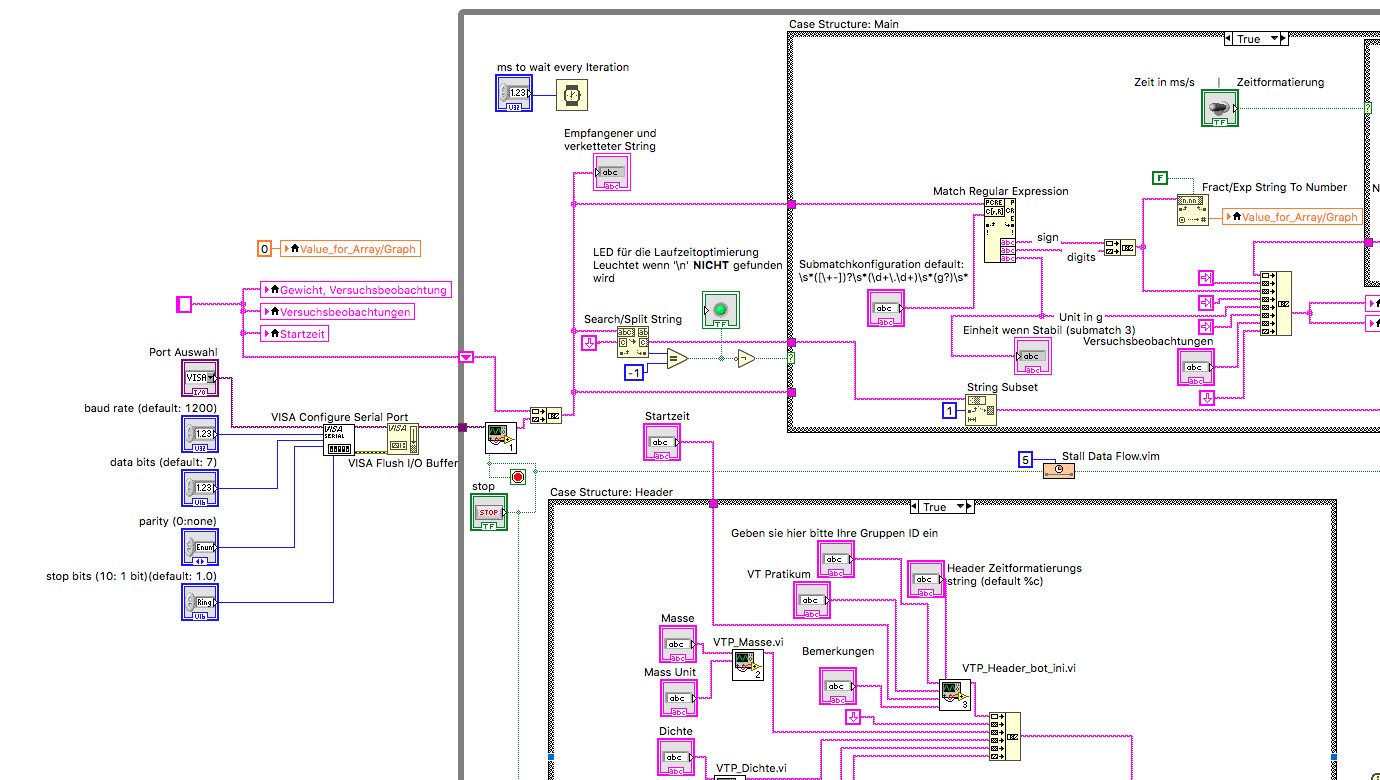
\includegraphics[height=0.3803\textwidth]
       {Bilder/LabVIEW_serialport/Haupt_VI_oben_links_2.jpg}
     }\hspace{-1.5pt}%\hfill     
    \subfloat[][oben rechts\label{fig:Haupt_VI_oben_rechts}]{%
       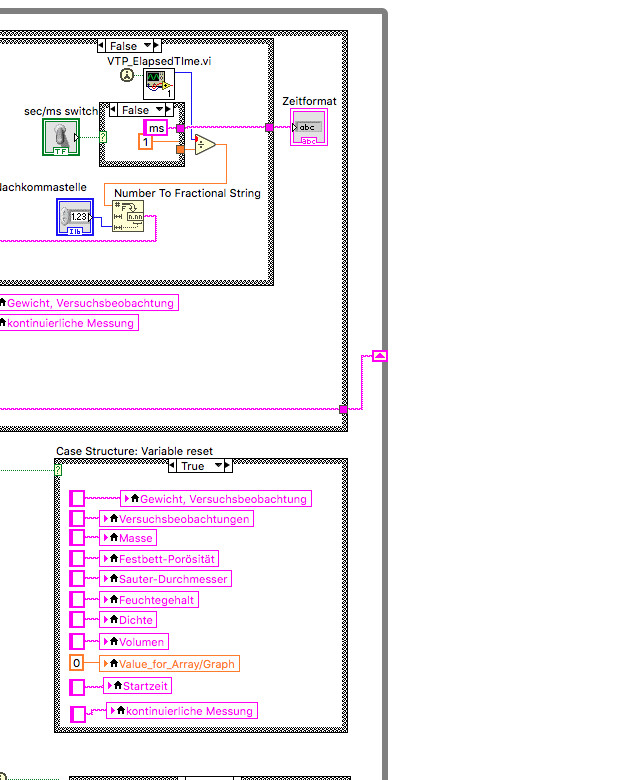
\includegraphics[height=0.3803\textwidth]
      {Bilder/LabVIEW_serialport/Haupt_VI_oben_rechts_2.jpg}
     }\phantomcaption
\vspace{-.81em}
\ContinuedFloat
\captionsetup{position=bottom}
\subfloat[position=top][unten links\label{fig:Haupt_VI_unten_links}]{%
       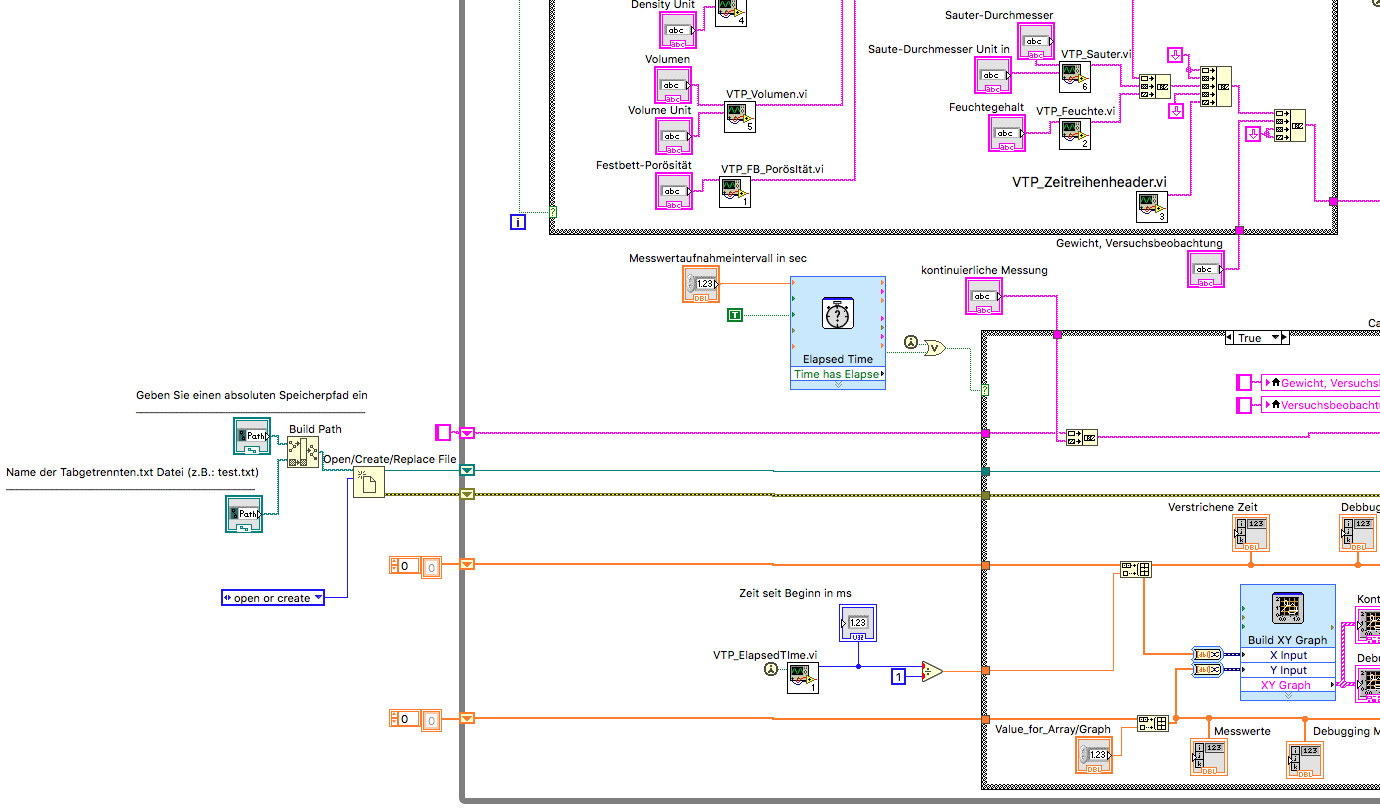
\includegraphics[height=0.395\textwidth]
       {Bilder/LabVIEW_serialport/Haupt_VI_unten_links_2.jpg}
     }\hspace{-1.6pt}%\hfill     
    \subfloat[position=top][unten rechts\label{fig:Haupt_VI_unten_rechts}]{%
       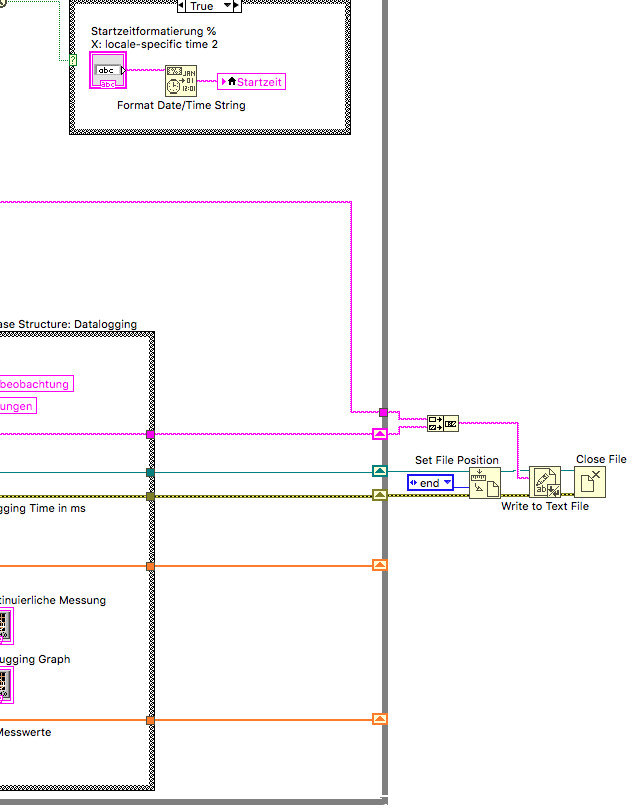
\includegraphics[height=0.395\textwidth]
      {Bilder/LabVIEW_serialport/Haupt_VI_unten_rechts_2.jpg}
     }    
\caption[Gesamtansicht des Haupt VI]{Gesamtansicht des Haupt VI}
\label{fig:Haupt_VI}
   \end{figure} 

\subparagraph*{Haupt VI Initialisierung}

%newpage
\begin{figure}[!h] % Haupt VI Initialisierung oben
\captionsetup{position=top}
\centering
\hspace{20mm}
     \subfloat[][Haupt VI Initialisierung: Variablen- und Portparametinitialisierung\label{haupt_ini_oben}]{%
       \includegraphics[width=0.6\textwidth]
       % {Bilder/LabVIEW_serialport/Dokumentheaderverkettung.jpg}
       {Bilder/LabVIEW_serialport/Haupt_VI_top_ini_2.jpg}
     }
    \phantomcaption
\vspace{-1.5em}
   \end{figure}
\begin{figure}[!h] % Haupt VI Initialisierung unten
\centering
\ContinuedFloat
\subfloat[][Haupt VI Initialisierung: Datalogger, Array und Stringinitialisierung\label{haupt_ini_unten}]{%
       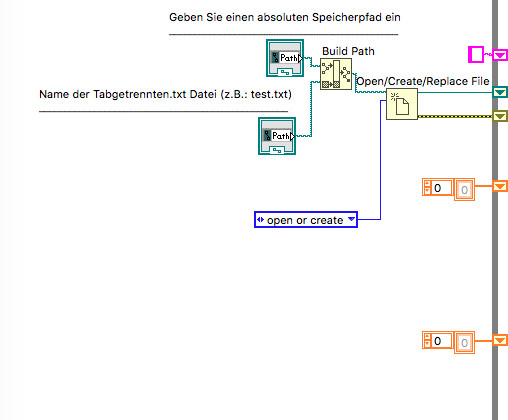
\includegraphics[width=0.6\textwidth]
        {Bilder/LabVIEW_serialport/Haupt_VI_ini_bot_2.jpg}
       }
\caption[Haupt VI Initialisierung \textbf{(a)} Teil 1 \textbf{(b)} Teil 2]{Haupt VI Initialisierung \textbf{(a)} Teil 1 \textbf{(b)} Teil 2}
\label{haupt_vi_ini}
   \end{figure}


Auf der Abbildung \ref{haupt_vi_ini} sind die Initialisierungen des \textit{While Loops} des Haupt VI's dargestellt. Es ist zu erkennen, dass der Port konfiguriert geöffnet und der Buffer einmal geflusht wird (siehe \ref{haupt_ini_oben}. In \ref{haupt_ini_unten} wird der absolute Dateipfad und der Dateiname aus der Frontpanel Eingabe übernommen. Wenn eine Datei mit dem Namen am angegebene Speicherort vorhanden ist, wird die Datei geöffnet (und unten anhängend beschrieben, siehe Abbildung \ref{fig:datalogger_rechts} oder \ref{datalogger} (38, 39)) wenn vorhanden oder neu erstellt. Des Weiteren ist zu erkennen, dass drei Arrays mit einem leeren Index 0  initialisiert werden.

\subparagraph*{Datalogger Initialisierung und Funktion}

 \begin{figure}[] % Datalogger Elapsed Time und Graph
 \centering
     \subfloat[][Messwert\-aufnahme\-intervall \textit{Control}\label{fig:datalogger_links}]{%
       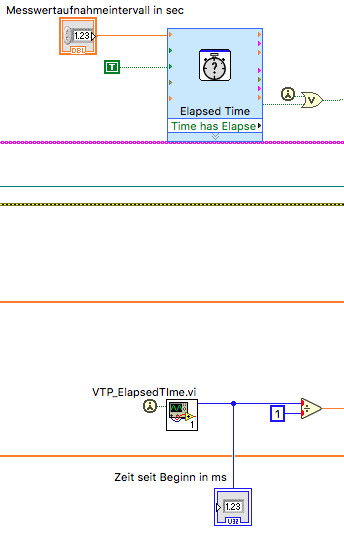
\includegraphics[height=0.57\textwidth]
       {Bilder/LabVIEW_serialport/datalogger_links.jpg}
     }
     \hspace{1pt}
\subfloat[][Datalaogger und Graphprogrammierung\label{fig:datalogger_rechts}]{%
       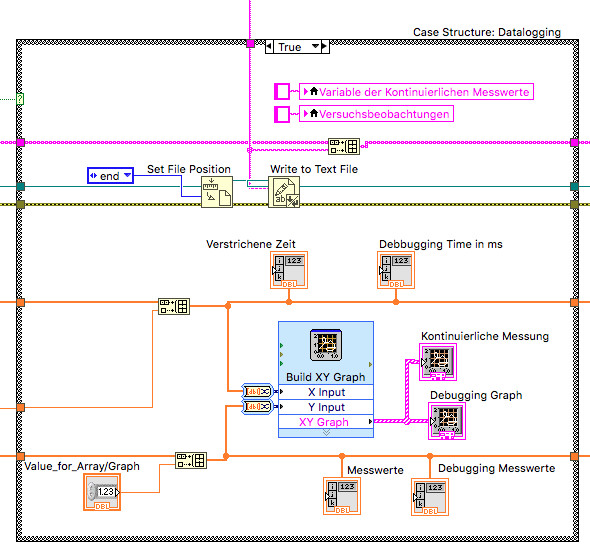
\includegraphics[height=0.57\textwidth]
      {Bilder/LabVIEW_serialport/datalogger_rechts.jpg}
       }
       \centering
\caption[Datalogger und Elapsed Time in ms \textbf{(a)} Messwert\-aufnahme\-intervall \textit{Control} 
\textbf{(b)} Datalaogger, Graphprogrammierung, Controleingabe löschen]
{Datalogger\,und\,Elapsed\,Time\,in\,ms \\
\textbf{(a)} Messwert\-aufnahme\-intervall \textit{Control} \\
\textbf{(b)} Datalaogger und Graphprogrammierung}
\label{datalogger_2}
 \end{figure}
 
Auf der Abbildung \ref{Haupt_Header_datawipe} ist in der linken \textit{Case Structure} die Konstruktion der Zeilen im \texttt{true} Case (wenn das Programm gestartet wird) zu erkennen. Der Header Satz wird so wie abgebildet in die Tabstoppgetrennte.txt Datei geschrieben. Spalteneinträge werden durch \texttt{Tabulator} (32) und Zeilen durch \texttt{Linefeed} (33) getrennt. Unten wird die Zeile mit den Messwerten und der Versuchsbeobachtung aus dem \textit{Variablenspeicher 1} (29) gelesen. Im \texttt{false} Case (wenn der Iterationsindex ungleich 0) werden die Daten direkt an die \textit{Case Structure: Datalogger} gesendet.\\

Rechts auf der Abbildung \ref{Haupt_Header_datawipe} ist die \textit{Case Structure: Variable Reset} zu erkennen. \textbf{Beim Beenden des Programms, werden alle Variablen gelöscht, die beim nächsten Programmstart wieder neu entgegen genommen werden sollen!}.
   
\bild{1}
{LabVIEW_serialport/Haupt_Header_datawipe.jpg}
{-1em}
{Modularer Header und \textit{Control} (Variablen) löschen bei Programmende}
{Modularer Header und \textit{Control} (Variablen) löschen bei Programmende}
{Haupt_Header_datawipe}


\subsubsection{Nutzen des VI`s}
\label{sec:Haupt_VI_Nutzung}

Damit dei Kommentarfunktion wie gewünscht funktioniert, ist vor der Verwendung des Programms in den LabVIEW Einstellungen unter Environment \glqq End Text entry with Enter key\grqq{} einzustellen (siehe Abbildung \ref{endtextentry}). Ist diese Option nicht eingestellt, muss nach jeder Betätigung der Enter-Taste, die Eingabe ein weiteres mal mittels eines Mausklicks auf einen schwarzen Haken, der neben dem VI Ausführen Pfeil (oben links im Front Panel) erscheint, quittiert werden.

\bild{0.7}
{LabVIEW_serialport/endtextentry.png}
{0em}
{Einstellung \glqq End text entry with Enter key\grqq{}}
{Einstellung \glqq End text entry with Enter key\grqq{}}
{endtextentry}

In den Abbildungen \ref{haupt_vi_start_eingaben}, \ref{haupt_vi_messung_konfiguration} und \ref{Haupt_VI_Debugging} ist zu erkennen, dass einige Optische veränderungen durch geführt worden sind. Es wurde eine \textit{Tab Control} verwendet, um verschiedene Register Fenster zu generieren, siehe folgende Liste:

\begin{itemize} % Haupt VI Reiter
\singlespacing
\item Start Einstellungen
\item Eingaben vor der Messung
\item Während der Messung
\item Konfiguration
\item Debugging
\end{itemize}

\begin{figure}[!h] % Haupt VI Starteinstellungen
\centering
     \subfloat[][Haupt VI Starteinstellungen
     \label{Haupt_VI_Starteinstellungen}]{%
       \includegraphics[width=1\textwidth]
       % {Bilder/LabVIEW_serialport/Dokumentheaderverkettung.jpg}
       {Bilder/LabVIEW_serialport/Haupt_VI_Starteinstellungen.jpg}
     }
    \phantomcaption
    % \caption[ #11]{#12}
    %\label{}
   \end{figure}
   
\begin{figure}[!h] % Haupt VI Eingaben
\centering
\ContinuedFloat
\subfloat[][Haupt VI Eingaben
		\label{Haupt_VI_Eingaben}]{%
       \includegraphics[width=1\textwidth]
        %{Bilder/LabVIEW_serialport/Dokumentheaderverkettung.jpg}
       {Bilder/LabVIEW_serialport/Haupt_VI_Eingaben.jpg}
       }
\caption[Haupt VI Starteinstellungen, Haupt VI Eingaben]{Haupt VI Starteinstellungen, Haupt VI Eingaben}
\label{haupt_vi_start_eingaben}
   \end{figure}
   
   \newpage
\begin{figure}[!h] % Haupt VI Messung
	\centering
     \subfloat[][Haupt VI Messung\label{Haupt_VI_Messung}]{%
       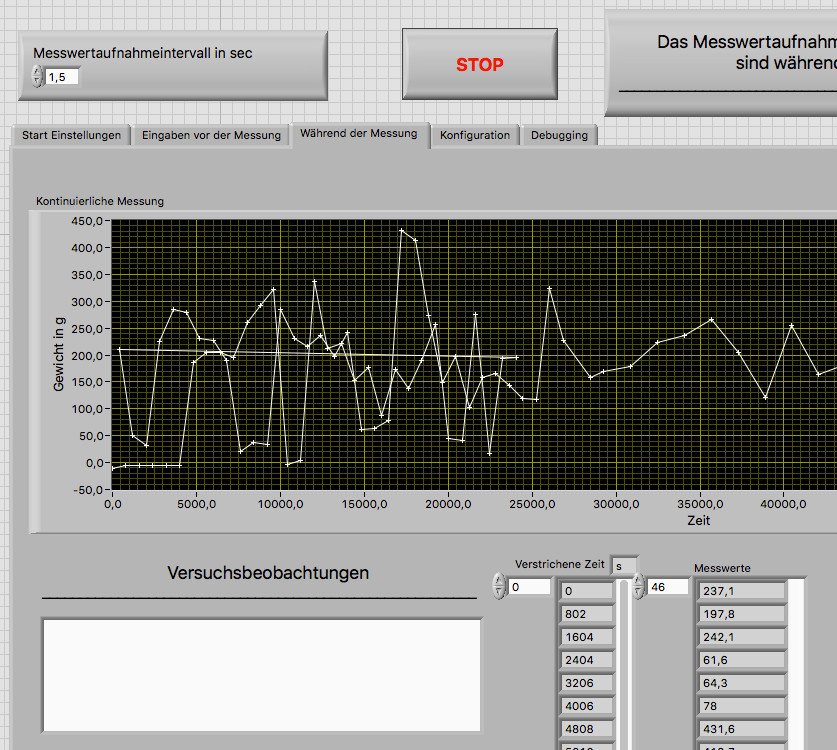
\includegraphics[width=0.48\textwidth]
       {Bilder/LabVIEW_serialport/Haupt_VI_Messung.jpg}
     }
     %\hfill
    \hspace{1mm}
\subfloat[][Haupt VI Konfiguration\label{Haupt_VI_Konfiguration}]{%
       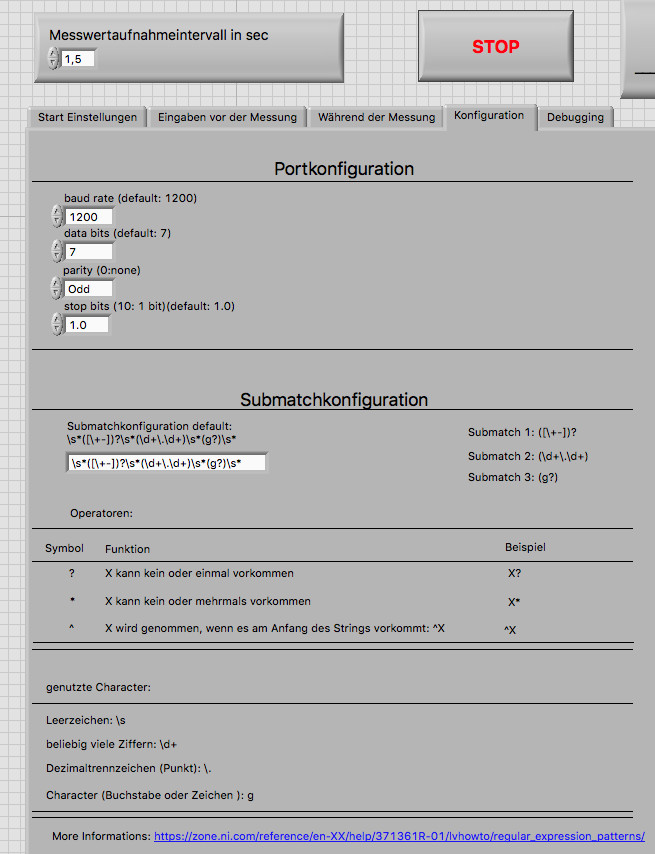
\includegraphics[width=0.49\textwidth]
       {Bilder/LabVIEW_serialport/Haupt_VI_Konfiguration}
       }
\caption[Haupt VI Messung, Haupt VI Konfiguration]{Haupt VI Messung, Haupt VI Konfiguration}
\label{haupt_vi_messung_konfiguration}
   \end{figure}
   
   \bild{1}
{LabVIEW_serialport/Haupt_VI_Debugging.jpg}
{-1em}
{Haupt VI Debugging}
{Haupt VI Debugging}
{Haupt_VI_Debugging}



 \bildp{h!}{0.7}
{LabVIEW_serialport/funktionstest.jpg}
{0em}
{Test aller Funktionen und Import in Excel}
{Test aller Funktionen und Import in Excel}
{funktionstest}

Auf der Abbildung \ref{funktionstest} ist zu erkennen, dass die Zeitstempelumschlatfunktion auch während der Messung funktioniert.


\subsubsection{Diskrete Messdatenerfassung RS-232}


Da die diskrete Messdatenerfassung nicht erwünscht ist, wird das vorgehen im folgenden kurz theoretisch beschrieben.

Um eine diskrete Messdatenerfassung zu realisieren, könnte der Messwert in ein Array geschrieben werden und mit den Wert(en) der Folgeiteration(en) verglichen werden. Als Abbruchbedingung des Programms könnte man definieren, dass wenn z.B. drei mal in Folge der gleiche Wert auftritt, der Wert in eine Datei geschrieben und das Programm beendet wird. Somit wäre gewährleistet, dass wenn zwei mal in Folge der gleiche fehlerhafte Wert auftritt (z.B. durch Paritätsfehler o.ä.) dieser nicht übernommen wird.

\subsection{DAQ mittels Messkarten}

Neben Geräten, die einen integrierten analog digital Wandler haben, gibt es Sensoren, die lediglich das analoge Signal transmittieren. Folglich muss das analoge Signal in ein digitales Signal umgewandelt werden. Für den Fall das Sensoren keinen integrierten analog/digital Wandler besitzen ist eine Messkarte zwischen Sensor und PC zu implementieren. \\


\begin{figure}[h!] %[htbp!] 
\centering
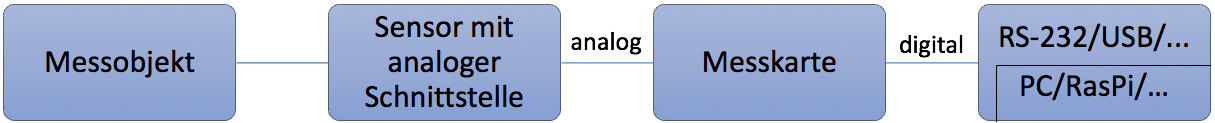
\includegraphics[width=1\textwidth]{Bilder/sensor_analoge_schnittstelle.jpg}
\vspace{0em}
 \caption[Messeinrichtungen mit integrierter digitaler Schnittstelle]{Messeinrichtungen mit integrierter digitaler Schnittstelle}\label{fig:sensor_digitale_schnittstelle}
\end{figure}

Im folgenden Abschnitt wird die DAQ eines Volumenstromsensors und eines Druckssensors mittels USB-6001 Messkarte von National Insturments erläutert .

\subsubsection{Kontinuierliche DAQ mittels NI-USB 6001}



\subsubsection{Diskrete DAQ mittels NI-USB 6001}

\subsection{Kontinuierliche Signale via RS-232 mit Python verarbeiten; Python Anaconda Spyder IDE}
text

%\subsubsection{}

\subsubsection{Benötigte Libraries}
text

\subsubsection{Beschreibung des Programmcodes... MatriX lässt Grüßen}
text

\subsection{Diskrete Signale via RS-232 mit Python verarbeiten}

